\documentclass[../notes.tex]{subfiles}

\pagestyle{main}
\renewcommand{\chaptermark}[1]{\markboth{\chaptername\ \thechapter\ (#1)}{}}
\setcounter{chapter}{2}

\begin{document}




\chapter{Energy and Angular Momentum}
\section{Energy and Conservative Forces in 3D; Angular Momentum}
\begin{itemize}
    \item \marginnote{10/6:}Recap.
    \begin{itemize}
        \item If $F(x,\dot{x},t)=F(x)$, then we can define $V(x)$.
        \item A bit more on kinetic, potential, and total energy in 1D.
    \end{itemize}
    \item Question: Is $\vec{F}(\vec{r},\dot{\vec{r}},t)=F(\vec{r})$ sufficient for the force to be conservative?
    \begin{itemize}
        \item Answer: No, it is not.
    \end{itemize}
    \item What \emph{is} a necessary and sufficient condition, then?
    \begin{itemize}
        \item If $T+V=E$, a constant, then we should have $\dv*{t}(T+V)=0$.
        \item Since
        \begin{align*}
            \dot{T} &= m(\dot{x}\ddot{x}+\dot{y}\ddot{y}+\dot{z}\ddot{z})
                = m\dot{\vec{r}}\cdot\ddot{\vec{r}}
                = \dot{\vec{r}}\cdot\vec{F}&
            \dot{V} &= \pdv{V}{x}\dot{x}+\pdv{V}{y}\dot{y}+\pdv{V}{z}\dot{z}
            = \dot{r}\cdot\vec{\nabla}V
        \end{align*}
        stating that $\dot{T}+\dot{V}=\dv*{t}(T+V)=0$ is equivalent to stating that
        \begin{equation*}
            \dot{\vec{r}}\cdot(\vec{F}+\vec{\nabla}V)
        \end{equation*}
        \item But from here, it follows that we must have $\vec{F}=-\vec{\nabla}V$.
        \item Takeaway: Conservative forces depend on $\vec{r}$ and can be written as $-\vec{\nabla}V$ for some scalar function $V$.
    \end{itemize}
    \item Can we express this condition more nicely? Yes!
    \begin{itemize}
        \item Claim: $\text{curl}\,(\vec{F})=\vec{\nabla}\times\vec{F}=0$ iff $\vec{F}=-\vec{\nabla}V$ for some scalar function $V$.
        \item Suppose $F=-\vec{\nabla}V$ for some scalar function $V$.
        \begin{itemize}
            \item Then since the curl of a gradient field is zero,
            \begin{equation*}
                \vec{\nabla}\times\vec{F} = \vec{\nabla}\times\vec{\nabla}V = 0
            \end{equation*}
        \end{itemize}
        \item Suppose $\vec{\nabla}\times\vec{F}=0$.
        \begin{itemize}
            \item To prove that $\vec{F}=-\vec{\nabla}V$ for some $V$, it will suffice to show that
            \begin{equation*}
                V(\vec{r}) = -\int_{\vec{r}_0}^{\vec{r}}\vec{F}\cdot\dd\vec{r'}
            \end{equation*}
            \item In particular, it will suffice to show that the function above is well defined. To do so, we will need to prove that the line integral on the right-hand side above is \textbf{path-independent}.
            \item But then by the equivalent path independence condition below, we need
            \begin{equation*}
                \oint_C\vec{F}\cdot\dd\vec{r} = 0
            \end{equation*}
            for all $C$.
            \item Applying \textbf{Stokes' theorem}, we obtain the equivalent condition
            \begin{equation*}
                \oint_C\vec{F}\cdot\dd\vec{r} = \iint_S(\vec{\nabla}\times\vec{F})\cdot\dd{\vec{S}} = \iint_S0\cdot\dd{\vec{S}} = 0
            \end{equation*}
            as desired.
        \end{itemize}
    \end{itemize}
    \item \textbf{Path-independent} (line integral): A line integral $\int_{\vec{r}_0}^{\vec{r}_1}\vec{A}\cdot\dd\vec{r}$ over some vector field $\vec{A}$ such that if $C_1,C_2$ are any two curves connecting $\vec{r}_0$ and $\vec{r}_1$, then
    \begin{equation*}
        \int_{C_1}\vec{A}\cdot\dd\vec{r} = \int_{C_2}\vec{A}\cdot\dd\vec{r}
    \end{equation*}
    \begin{figure}[h!]
        \centering
        \begin{tikzpicture}
            \footnotesize
            \draw [stealth-stealth] (0,3) -- (0,0) -- (3.5,0);
    
            \draw [help lines, ->] (0.5,0.8) -- ++(0.3,0.3);
            \draw [help lines, ->] (0.2,2.2) -- ++(0.3,0.3);
            \draw [help lines, ->] (1,0.3) -- ++(0.3,0.3);
            \draw [help lines, ->] (0.8,2) -- ++(0.3,0.3);
            \draw [help lines, ->] (1.4,1.5) -- ++(0.3,0.3);
            \draw [help lines, ->] (1.2,2.5) -- ++(0.3,0.3);
            \draw [help lines, ->] (1.8,1.2) -- ++(0.3,0.3);
            \draw [help lines, ->] (2.3,0.4) -- ++(0.3,0.3);
            \draw [help lines, ->] (2.4,2.2) -- ++(0.3,0.3);
            \draw [help lines, ->] (2.5,1) -- ++(0.3,0.3);
    
            \draw [pux,thick]
                (0.9,0.8) .. controls (3,0.5) and (2,2) .. node[near start,below=2pt]{$C_1$} (2.4,2.7)
                (0.9,0.8) .. controls (0.8,3) and (2,2) .. node[near end,above=2pt]{$C_2$} (2.4,2.7)
            ;
    
            \fill (0.9,0.8) circle (2pt) node[below left]{$\vec{r}_0$};
            \fill (2.4,2.7) circle (2pt) node[above right]{$\vec{r}_1$};
        \end{tikzpicture}
        \caption{Path independent line integral.}
        \label{fig:pathIndependent}
    \end{figure}
    \begin{itemize}
        \item An equivalent path independence condition may be obtained via inspection of Figure \ref{fig:pathIndependent}.
        \item Indeed, saying that the path integral along $C_1$ (from $\vec{r}_0$ to $\vec{r}_1$) equals that along $C_2$ (from $\vec{r}_0$ to $\vec{r}_1$) is equivalent to saying that the difference of the path integrals is equal to zero. Equivalently, the path integral along $C_1$ (from $\vec{r}_0$ to $\vec{r}_1$) plus the path integral along $C_2$ (from $\vec{r}_1$ to $\vec{r}_0$) equals zero. But this sum of path integrals is just the closed loop integral $\oint_C$ around the oriented curve $C=C_1-C_2$.
        \item Thus, equivalently,
        \begin{equation*}
            \int_C\vec{A}\cdot\dd\vec{r} = 0
        \end{equation*}
        for all $C$ containing $\vec{r}_0$ and $\vec{r}_1$.
        \item Lastly, note that we do not need to constrain the curves to $\vec{r}_0$ and $\vec{r}_1$ but can let them freely range over the whole space. Thus, we can check the closed loop integral over all loops $C$ in the space.
    \end{itemize}
    \item \textbf{Stokes' theorem}: The following integral equality, where $C$ is a closed curve bounding the curved surface $S$ and $\vec{A}$ is a vector field. \emph{Given by}
    \begin{equation*}
        \oint_C\vec{F}\cdot\dd\vec{r} = \iint_S(\vec{\nabla}\times\vec{A})\cdot\dd{\vec{S}}
    \end{equation*}
    \item How do we find $V$ from $F$?
    \begin{itemize}
        \item First, we need an integral theorem.
        \item Theorem: For all scalar functions $\phi:\mathbb{R}^3\to\mathbb{R}$ defining conservative forces and all points $\vec{r}_0,\vec{r}_1\in\mathbb{R}^3$, the \textbf{line integral}
        \begin{equation*}
            \int_{\vec{r}_0}^{\vec{r}_1}\vec{\nabla}\phi\cdot\dd\vec{r} = \phi(\vec{r}_1)-\phi(\vec{r}_0)
        \end{equation*}
        \item It follows that if $F=-\nabla V$, then
        \begin{equation*}
            V(\vec{r}_1)-V(\vec{r}_0) = -\int_{\vec{r}_0}^{\vec{r}_1}\vec{\nabla}V\cdot\dd\vec{r}
        \end{equation*}
    \end{itemize}
    \item We now move onto rotation.
    \begin{itemize}
        \item We describe rotation in polar coordinates.
        \item Let $\ell_r$ be the length in the radial direction, and let $\ell_\theta$ be the length in the angular direction.
        \item Then
        \begin{align*}
            \dd\ell_r &= \dd{r}&
            \dd\ell_\theta &= r\dd\theta
        \end{align*}
        where
        \begin{align*}
            \hat{r} &= \ihat\cos\theta+\jhat\sin\theta&
            \hat{\theta} &= -\ihat\sin\theta+\jhat\cos\theta
        \end{align*}
        \item Coordinate-wise, we have
        \begin{align*}
            x &= r\cos\theta&
            y &= r\sin\theta
        \end{align*}
        \item Velocity-wise, we have $\vec{v}=v_x\ihat+v_y\jhat$ where
        \begin{align*}
            v_x &= \dot{r}\cos\theta-r\dot{\theta}\sin\theta&
                v_y &= \dot{r}\sin\theta+r\dot{\theta}\cos\theta\\
            v_r &= \vec{v}\cdot\hat{r} = \dot{r} = \dv{\ell_r}{t}&
                v_\theta &= \vec{v}\cdot\hat{\theta} = r\dot{\theta} = \dv{\ell_\theta}{t}
        \end{align*}
    \end{itemize}
    \item The analogy of force under rotation is \textbf{torque}.
    \item \textbf{Torque}: A twisting force that tends to cause rotation, quantified as follows. \emph{Also known as} \textbf{moment of force}. \emph{Denoted by} $\bm{\vec{g}}$. \emph{Given by}
    \begin{equation*}
        \vec{G} = \vec{r}\times\vec{F}
    \end{equation*}
    \begin{itemize}
        \item Componentwise, we have
        \begin{align*}
            G_x &= yF_z-zF_y&
            G_y &= zF_x-xF_z&
            G_z &= xF_y-yF_x
        \end{align*}
        \item We also have $\norm{\vec{G}}=rF\sin\theta$.
    \end{itemize}
    \item Momentum under rotation: Angular momentum.
    \item \textbf{Angular momentum}: The quantity of rotation of a body, quantified as follows. \emph{Denoted by} $\bm{\vec{J}}$. \emph{Given by}
    \begin{equation*}
        \vec{J} = \vec{r}\times\vec{p}
        = m\vec{r}\times\vec{r}
    \end{equation*}
    \begin{itemize}
        \item Derivative:
        \begin{equation*}
            \dot{\vec{J}} = \vec{G}
        \end{equation*}
    \end{itemize}
    \item \textbf{Central force}: A force that flows toward or away from the origin, i.e., is in the $\hat{r}$ direction.
    \begin{itemize}
        \item Identify with $\vec{r}\times\vec{F}=0$.
    \end{itemize}
    \item Under central forces, angular momentum is conserved.
    \begin{itemize}
        \item We have
        \begin{equation*}
            \vec{J} = mr^2\dot{\theta}\hat{z}
        \end{equation*}
        \item Sweeping out equal areas (Kepler's 2nd law): We have
        \begin{align*}
            \dd{A} &= \frac{1}{2}r^2\dd{\theta} = \pi r^2\frac{\dd{\theta}}{2\pi}\\
            \dv{A}{t} &= \frac{1}{2}r^2\dot{\theta}
        \end{align*}
    \end{itemize}
\end{itemize}



\section{Introduction to Variational Calculus and the Lagrangian}
\begin{itemize}
    \item \marginnote{10/9:}Recap points from last time, then variational calculus (different form of mechanics that is more powerful than Newton's laws, called Lagrangian mechanics).
    \item One particle feeling external conservative forces.
    \item We'll revisit this later when we learn Hamiltonian mechanics.
    \item Suppose we have one particle in three dimensions.
    \begin{itemize}
        \item Newton tells us that we can get EOM by figuring out all the forces on each particle and setting the net force equal to the mass times acceleration.
        \item This is often written componentwise.
        \item For the special case of a conservative force (requirement is that the curl vanishes, $\vec{\nabla}\times\vec{F}=0$), we can find a scalar potential energy function $V$ such that $\vec{F}=-\vec{\nabla}V$.
        \item Each
        \begin{equation*}
            -\pdv{V}{x_i} = F_i = m\vec{\ddot{r}}_i = \dot{p}_i
        \end{equation*}
    \end{itemize}
    \item Intro to variational calculus.
    \begin{itemize}
        \item We're not responsible for doing variational calculations, themselves, but we will use the results.
    \end{itemize}
    \item The variational problem.
    \begin{itemize}
        \item Define a family of curves in the space $t\oplus x$ connecting two points $(t_0,x_0)$ and $(t_1,x_1)$.
        \item We have a \textbf{functional}
        \begin{equation*}
            \Phi = \int_{t_0}^{t_1}f(x(t),\dot{x}(t),t)\dd{t}
        \end{equation*}
        \item The problem: Find the path $x(t)$ that makes $\Phi$ into an extremum (i.e., minimum or maximum).
        \item Example: Find the curve that minimizes the distance between the two points.
    \end{itemize}
    \item \textbf{Functional}: A function of curves (as opposed to points or values).
    \item Solving such problems.
    \begin{itemize}
        \item We want to find a way to differentiate functionals like $\Phi$ with respect to curves.
        \item Let $x(t)$ be the curve for which $\Phi$ is minimal or maximal (aka extremal or \textbf{stationary}).
        \item Let $\eta(t)$ be any smooth function with $\eta(t_0)=\eta(t_1)=0$.
        \item Define $x(t,0)=x(t)$ and $x(t,\alpha)=x(t,0)+\alpha\eta(t)$.
        \item Now, we can write $\Phi$ as a function of $\alpha$!
        \begin{equation*}
            \Phi(\alpha) = \int_{t_0}^{t_1}f(x(t,\alpha),\dot{x}(t,\alpha),t)\dd{t}
        \end{equation*}
        \item For $x(t)$ to be an extremum, we need
        \begin{equation*}
            \eval{\pdv{\Phi}{\alpha}}_{\alpha=0} = 0
        \end{equation*}
        for all $\eta(t)$.
        \item Now we take
        \begin{align*}
            \pdv{\Phi}{\alpha} &= \pdv{\alpha}\int_{t_0}^{t_1}f(x,\dot{x},t)\dd{t}\\
            &= \int_{t_0}^{t_1}\pdv{f}{\alpha}(x,\dot{x},t)\dd{t}\\
            &= \int_{t_0}^{t_1}\left( \pdv{f}{x}\pdv{x}{\alpha}+\pdv{f}{\dot{x}}\pdv{\dot{x}}{\alpha} \right)\dd{t}
        \end{align*}
        \item But we have that
        \begin{align*}
            x(t,\alpha) &= x(t)+\alpha\eta(t)&
            \dot{x}(t,\alpha) &= \dot{x}(t)+\alpha\dot{\eta}(t)
        \end{align*}
        so
        \begin{align*}
            \pdv{x}{\alpha} &= \eta(t)&
            \pdv{\dot{x}}{\alpha} &= \dot{\eta}(t)
        \end{align*}
        \item Thus, continuing from the above,
        \begin{equation*}
            \pdv{\Phi}{\alpha} = \int_{t_0}^{t_1}\left( \pdv{f}{x}\eta(t)+\pdv{f}{\dot{x}}\pdv{\eta}{t} \right)\dd{t}
        \end{equation*}
        \item We now integrate by parts.
        \begin{equation*}
            \int_{t_0}^{t_1}\pdv{f}{\dot{x}}\dv{\eta}{t}\dd{t} = \pdv{f}{\dot{x}}[\eta(t_1)-\eta(t_0)]-\int_{t_0}^{t_1}\dv{t}(\pdv{f}{\dot{x}})\eta(t)\dd{t}
        \end{equation*}
        \item The first term after the equals sign goes to zero by the definition of $\eta$.
        \item Thus, continuing from the above,
        \begin{align*}
            \pdv{\Phi}{\alpha} &= \int_{t_0}^{t_1}\left( \pdv{f}{x}\eta(t)-\dv{t}(\pdv{f}{\dot{x}})\eta(t) \right)\dd{t}\\
            &= \int_{t_0}^{t_1}\left( \pdv{f}{x}-\dv{t}(\pdv{f}{\dot{x}}) \right)\eta(t)\dd{t}
        \end{align*}
        \item Thus, since we want $\pdv*{\Phi}{\alpha}|_{\alpha=0}=0$, our condition that $f$ must satisfy is
        \begin{equation*}
            \int_{t_0}^{t_1}\left( \pdv{f}{x}-\dv{t}(\pdv{f}{\dot{x}}) \right)\eta(t)\dd{t} = 0
        \end{equation*}
        for any $\eta(t)$.
        \item In particular, if this is to be zero for all $\eta(t)$, then we must have
        \begin{equation*}
            \pdv{f}{x}-\dv{t}(\pdv{f}{\dot{x}}) = 0
        \end{equation*}
        \item This is called an \textbf{Euler Equation} within mathematics, and an \textbf{Euler-Lagrange Equation} within physics.
    \end{itemize}
    \item Variational example: What shape of curve minimizes the distance between two points.
    \begin{itemize}
        \item In the plane, we all know that this is a straight line, and we will prove this now.
        \begin{itemize}
            \item Aside: The problem is more interesting when applied to curved surfaces, such as geodesics or the sphere (great circle routes).
        \end{itemize}
        \item Recall that $\dd{\ell}=\sqrt{\dd{t}^2+\dd{x}^2}=\dd{t}\sqrt{1+\dot{x}^2}$.
        \item We want to minimize the sum of these distances along the curve (arc length), i.e., we want to minimize
        \begin{equation*}
            \Phi = \int_{t_0}^{t_1}\dd{t}\sqrt{1+\dot{x}^2}
        \end{equation*}
        \item From here, we may define
        \begin{equation*}
            f(x,\dot{x},t) = \sqrt{1+\dot{x}^2}
        \end{equation*}
        for substitution into the Euler-Lagrange equation.
        \item Substituting, we obtain
        \begin{align*}
            \dv{t}(\pdv{f}{\dot{x}}) &= \pdv{f}{x}\\
            \dv{t}(\frac{1}{2}(1+\dot{x}^2)^{-1/2}(2\dot{x})) &= 0\\
            \dv{t}(\frac{\dot{x}}{\sqrt{1+\dot{x}^2}}) &= 0\\
            \frac{\dot{x}}{\sqrt{1+\dot{x}^2}} &= C
        \end{align*}
        \item If the whole final expression is constant, then it must be that $\dot{x}$ is constant. From here, we can recover $x(t)=ct+b$.
        \item Note that we have not proven that this is the minimum (it could be a maximum of $\Phi$!). But \emph{if} there is a minimum, it is this.
    \end{itemize}
    \item In 3D, we can consider an equation of the form $f(x_1,x_2,x_3,\dot{x}_1,\dot{x}_2,\dot{x}_3,t)$.
    \begin{itemize}
        \item Running this back through the procedure, we get an Euler-Lagrange equation for each component.
        \begin{equation*}
            \pdv{f}{x_i}-\dv{t}(\pdv{f}{\dot{x}_i}) = 0
        \end{equation*}
    \end{itemize}
    \item We want a variational form of Newton's laws.
    \begin{itemize}
        \item Compare the Euler-Lagrange equation and an analogous form of Newton's law.
        \begin{align*}
            \dv{t}(\pdv{f}{\dot{x}_i}) &= \pdv{f}{x_i}&
            \dv{t}(m\dot{x}_i) &= -\pdv{V}{x_i}
        \end{align*}
        \item Let
        \begin{equation*}
            f = T-V
            = \sum_i\frac{1}{2}m\dot{x}_i^2-V(\{x_i\})
        \end{equation*}
        where $V(\{x_i\})$ denotes $V(x_1,x_2,x_3)$.
    \end{itemize}
    \item \textbf{Lagrangian function}: The function defined as follows. \emph{Denoted by} $\bm{L}$. \emph{Given by}
    \begin{equation*}
        L = T-V
    \end{equation*}
    \item \textbf{Action}: The following integral. \emph{Also known as} \textbf{action integral}. \emph{Denoted by} $\bm{S}$, $\bm{I}$. \emph{Given by}
    \begin{equation*}
        S = \int_{t_0}^{t_1}L(x_i,\dot{x}_i,t)\dd{t}
    \end{equation*}
    \item \textbf{Least action principle}: Particle trajectories are those for which $S$ is extremal.
    \begin{itemize}
        \item Not always needed or necessary.
    \end{itemize}
    \item Procedure for finding equations of motion.
    \begin{enumerate}
        \item Write down your Lagrangian for the system.
        \item Use the componentwise Euler-Lagrange equations to find the EOMs.
    \end{enumerate}
    \item Why do this?
    \begin{enumerate}
        \item We can use any coordinate system to define $L$.
        \begin{itemize}
            \item It's often easier to change coordinates at the stage of scalar functions rather than later when you're dealing with multiple derivatives, vectors, etc.
        \end{itemize}
        \item Much easier to specify constraints.
        \begin{itemize}
            \item We can also use this formalism (as we'll see next time) to go backwards and see what the original forces are.
        \end{itemize}
        \item Symmetries and conservation laws are often more transparent in this formulation.
    \end{enumerate}
    \item Example.
    \begin{itemize}
        \item Suppose we have a bead that is constrained to move under gravity along a parabolic wire.
        \item Let the equation of the wire be $z=ax^2$.
        \item The wire exerts normal forces; it's hard to figure out what these are because the curvature of the wire is constantly changing.
        \item Write
        \begin{align*}
            T &= \frac{1}{2}m(\dot{x}^2+\dot{z}^2)&
            V &= mgz
        \end{align*}
        \item We also need $\dot{z}=2ax\dot{x}$.
        \item Thus,
        \begin{align*}
            L &= T-V\\
            &= \frac{1}{2}m(\dot{x}^2+(2ax\dot{x})^2)-mgax^2\\
            &= \frac{1}{2}m(\dot{x}^2+4a^2x^2\dot{x}^2)-mgax^2
        \end{align*}
        \item We can now find the equations of motion with the Euler-Lagrange equation.
        \begin{align*}
            \dv{t}(\pdv{L}{\dot{x}}) &= \pdv{L}{x}\\
            \dv{t}(m\dot{x}+4ma^2x^2\dot{x}) &= 4ma^2x\dot{x}^2-2mgax\\
            m\ddot{x}+8ma^2x\dot{x}^2+4ma^2x^2\ddot{x} &= 4ma^2x\dot{x}^2-2mgax\\
            % \ddot{x}+4a^2(x\dot{x}^2+x^2\ddot{x})+2gax &= 0\\
            \ddot{x}(1+4a^2x^2)+\dot{x}^2(4a^2x)+2gax &= 0
        \end{align*}
        \item This final expression is pretty complicated! It would have been very complicated (perhaps prohibitively so) to arrive here with kinematics.
    \end{itemize}
    \item Imagine now that this wire is rotating at constant angular velocity $\omega$.
    \begin{itemize}
        \item We can solve this in rotating coordinates just as easily!
        \item This time, take
        \begin{equation*}
            T = \frac{1}{2}m(v_r^2+v_\theta^2+v_z^2)
        \end{equation*}
        where
        \begin{align*}
            v_r &= \dot{r}&
            v_\theta &= r\dot{\theta} = r\omega&
            v_z &= \dot{z}
        \end{align*}
    \end{itemize}
\end{itemize}



\section{Office Hours (Jerison)}
\begin{itemize}
    \item Phase offsets in the driven harmonic oscillator.
\end{itemize}



\section{Introduction to the Lagrangian: Examples and the Free Particle}
\begin{itemize}
    \item \marginnote{10/11:}Now that we have the Lagrangian, pretty soon, we will be able to prove why the kinetic energy has the form $mv^2/2$.
    \begin{itemize}
        \item We won't be required to reproduce this derivation, though.
    \end{itemize}
    \item Announcements.
    \begin{itemize}
        \item Midterm will be on a Wednesday during our section.
        \item No pset due Friday of midterm week; a smaller one will be due the following Monday.
        \item There will be another small one due that Friday.
        \item Some textbook chapters have been posted on Canvas with more background on the Lagrangian; they contain info that may be helpful for our homework.
    \end{itemize}
    \item Today: Pendulum and generalized coordinates.
    \item Next time: Lagrange multipliers and constraints; start central, conservative forces.
    \item Recap.
    \begin{itemize}
        \item $L=T-V=T(\{q_i\})-V(\{q_i\})$.
        \begin{itemize}
            \item We use $q$ instead of $x$ because these coordinates don't have to be positions!
        \end{itemize}
        \item Lagrange's equations of motion:
        \begin{equation*}
            \dv{t}(\pdv{L}{\dot{q}_i}) = \pdv{L}{q_i}
        \end{equation*}
        for $i=1,2,3$ for an unconstrained particle.
        \item Why use Lagrangian mechanics?
        \begin{enumerate}
            \item Constraints are easy to incorporate, e.g., bead on a quadratic wire.
            \item We can choose any generalized coordinates in which to express $T,V$.
            \item Symmetries are often more transparent.
        \end{enumerate}
        \item We talked about 1 last time; we'll talk about 2-3 today.
    \end{itemize}
    \item Generalized coordinates.
    \item Example (use of different coordinates): Simple pendulum.
    \begin{figure}[h!]
        \centering
        \begin{tikzpicture}
            \footnotesize
            \draw [dashed]
                (0,2.5) -- (0,-1) coordinate (A)
                (-1.5,2) -- (1.5,2)
            ;
    
            \draw [->] (1,0) -- ++(270:0.8) node[above left]{$mg$};
            \draw [->] (1,0) -- ++(300:0.6) node[below right=-1pt]{$\hat{r}$};
            \draw [->] (1,0) -- ++(30:0.6) node[above right=-1pt]{$\hat{\theta}$};
    
            \draw [gry,thick] (0,2) coordinate (B) node[circle,fill,black,inner sep=1pt,label={[above right=-1pt,black]$(0,0)$}]{} -- node[above right=-1pt,black]{$\ell$} (1,0) coordinate (C) node[circle,fill,grx,inner sep=2pt,label={[below right=1pt,black]m}]{} pic [draw,black,thin,angle radius=7mm,angle eccentricity=1.2,pic text={$\theta$}] {angle=A--B--C};
        \end{tikzpicture}
        \caption{Simple pendulum.}
        \label{fig:simplePendulum}
    \end{figure}
    \begin{itemize}
        \item A rigid, massless rod of length $\ell$ pinned at the top and connected to a bob of mass $m$ that makes angle $\theta$ with the vertical.
        \item EOM with Newton's laws.
        \begin{itemize}
            \item $\vec{F}=m\ddot{\vec{r}}$.
            \item This system has a plane polar symmetry, so we want an expression in plane polar coordinates.
            \item In particular, in these coordinates, $\ddot{\vec{r}}=(\ddot{r}-r\dot{\theta}^2)\hat{r}+(r\ddot{\theta}+2\dot{r}\dot{\theta})\hat{\theta}$.
            \item Using this acceleration vector, the EOMs are as follows:
            \begin{align*}
                F_{T,\text{rod}}+mg\cos\theta &= F_r = m(\ddot{r}-r\dot{\theta}^2)&
                -mg\sin\theta &= F_\theta = m(r\ddot{\theta}+2\dot{r}\dot{\theta})
            \end{align*}
            \item We know by inspection of Figure \ref{fig:simplePendulum} that $\ddot{r}=\dot{r}=0$ and $r=\ell$, so the above becomes
            \begin{align*}
                F_r &= -m\ell\dot{\theta}^2&
                F_\theta &= m\ell\ddot{\theta}
            \end{align*}
            \item Since the radial forces are balanced, we only need to worry about the angular ones going forward. In particular, by transitivity, the final EOM is
            \begin{align*}
                m\ell\ddot{\theta} &= -mg\sin\theta\\
                \ddot{\theta} &= -\frac{g}{\ell}\sin\theta
            \end{align*}
            as desired.
        \end{itemize}
        \item EOM with the Lagrangian.
        \begin{itemize}
            \item $L=T-V$, where
            \begin{align*}
                T &= \frac{1}{2}m(v_r^2+v_\theta^2)
                    = \frac{1}{2}m(\dot{r}^2+r^2\dot{\theta}^2)
                    = \frac{1}{2}m\ell^2\dot{\theta}^2&
                V &= -mg\ell\cos\theta
            \end{align*}
            \item Note that we can define the potential energy function as such instead of as $mg(\ell-\ell\cos\theta)$ since we may choose the zero of potential energy to be $mg\ell$!
            \item Thus, the complete Lagrangian is
            \begin{equation*}
                L = \frac{1}{2}m\ell^2\dot{\theta}^2+mg\ell\cos\theta
            \end{equation*}
            \item With only one of the two coordinates remaining (that is, $\theta$ not $r$), we only need an Euler-Lagrange equation in this one component to find the complete EOM:
            \begin{align*}
                \dv{t}(\pdv{L}{\dot{\theta}}) &= \pdv{L}{\theta}\\
                \dv{t}(m\ell^2\dot{\theta}) &= -mg\ell\sin\theta\\
                m\ell^2\ddot{\theta} &= -mg\ell\sin\theta\\
                \ddot{\theta} &= -\frac{g}{\ell}\sin\theta
            \end{align*}
        \end{itemize}
        \item Thus, we got the same result without having to derive the complicated transformation between Cartesian and polar coordinates!
    \end{itemize}
    \item The $\theta$ above is the first example we've seen thus far of a \textbf{generalized coordinate} (we'll see further examples later).
    \item $\pdv*{L}{\dot{q}_i}$ is often referred to as a \textbf{generalized momentum} and $\pdv*{L}{q_i}$ is often referred to as a \textbf{generalized force}.
    \begin{itemize}
        \item If we're in Cartesian coordinates, these things are \emph{actual} momenta and forces since\dots
        \begin{align*}
            \pdv{L}{\dot{x}_i} &= m\dot{x}_i
                = p_i&
            \pdv{L}{x_i} &= -\dv{V}{x_i}
                = F_i
        \end{align*}
        \item In the case of the pendulum, recall that we have
        \begin{align*}
            \pdv{L}{\dot{\theta}} &= m\ell^2\dot{\theta}&
            \pdv{L}{\theta} &= -mg\ell\sin\theta
        \end{align*}
        \begin{itemize}
            \item The left one can be recognized as the angular momentum $\vec{r}\times\vec{p}$.
            \item The right one can be recognized as the torque $\vec{r}\times\vec{F}$.
        \end{itemize}
        \item If $L$ is independent of $q_i$ for some $q_i$, then $\pdv*{L}{\dot{q}_i}$ is constant in time and hence we have a conserved force (in some sense).
        \begin{itemize}
            \item In particular, if $L$ is independent of some $q_i$, then $0=\pdv*{L}{q_i}=\dv*{t}(\pdv*{L}{\dot{q}_i})$, so $\pdv*{L}{\dot{q}_i}$ is constant in time.
        \end{itemize}
    \end{itemize}
    \item One last thing to keep in mind about coordinate systems.
    \item Cylindrical and spherical coordinates.
    \begin{itemize}
        \item Cylindrical:
        \begin{align*}
            x &= r\cos\phi&
            y &= r\sin\phi&
            z &= z
        \end{align*}
        \item Spherical:
        \begin{align*}
            x &= r\sin\theta\cos\phi&
            y &= r\sin\theta\sin\phi&
            z &= r\cos\theta
        \end{align*}
        \begin{itemize}
            \item In this case, $\theta$ comes down from the vertical, and $\phi$ sweeps around the $xy$-plane.
            \item Thus, $\theta=[0,\pi]$ and $\phi=[0,2\pi]$.
        \end{itemize}
    \end{itemize}
    \item Moving on: Symmetries.
    \item Why is $T=mv^2/2$? Let's look at the Lagrangian of a \textbf{free particle}.
    \begin{itemize}
        \item No external forces means that $V=0$ and thus $L=T-0=T$.
        \item If we believe Galileo's relativity principle, then the EOMs must be the same in any inertial reference frame.
        \item This is \emph{almost} the same as saying that the Lagrangian must be the same in any inertial reference frame, but not quite!
        \item In particular, if $L'=L+\dv*{t}f(q_i,t)$, then $L'$ and $L$ give the same EOMs, that is, they are equivalent.
        \begin{itemize}
            \item Note: We have just defined a notion of \emph{equivalence} for Lagrangians!
        \end{itemize}
        \item To see that they do give the same EOMs, start by expanding the definition of $L'$ above.
        \begin{equation*}
            L' = L+\sum_i\pdv{f}{q_i}\dot{q}_i+\pdv{f}{t}
        \end{equation*}
        \item Next, observe that
        \begin{align*}
            \pdv{L'}{\dot{q}_i} &= \pdv{L}{\dot{q}_i}+\pdv{f}{q_i}&
            \pdv{L'}{q_i} &= \pdv{L}{q_i}+\dv{t}(\pdv{f}{q_i})
        \end{align*}
        \begin{itemize}
            \item For the left equation above, we use the facts that $L$ may have a $\dot{q}_i$ term, $\pdv*{f}{q_i}\dot{q_i}$ does have a $\dot{q}_i$, and every other term does not contain a $\dot{q}_i$. This allows us to compute the partial derivative as written.
            \item For the right equation above, note that the partial and total derivatives $\pdv*{q_i}$ and $\dv*{t}$ do not commute in general. However, in this case, we know that
            \begin{equation*}
                \pdv{q_i}(\sum_j\pdv{f}{q_j}\dot{q}_j+\pdv{f}{t}) = \sum_i\dot{q}_j\cdot\pdv{j}\pdv{f}{q_i}+\pdv{t}\pdv{f}{q_i}
                = \dd{t}(\pdv{f}{q_i})
            \end{equation*}
            But how come $\pdv{q_i}\pdv{f}{q_j}\dot{q}_j=\dot{q}_j\cdot\pdv{j}\pdv{f}{q_i}$?? How do we know that $\dot{q}_j$ does not depend on $q_i$?
        \end{itemize}
        \item Last, it follows that the EOMs from $L'$ are
        \begin{align*}
            \dv{t}(\pdv{L}{\dot{q}_i}+\pdv{f}{q_i}) &= \pdv{L}{q_i}+\dv{t}\pdv{f}{q_i}\\
            \dv{t}(\pdv{L}{\dot{q}_i}) &= \pdv{L}{q_i}
        \end{align*}
        i.e., are the same as those from $L$, as desired.
    \end{itemize}
    \item \textbf{Free particle}: A particle moving with some velocity $v$ in a reference frame $K$ under the influence of no external forces.
    \item A teaser for next time.
    \begin{itemize}
        \item Suppose we have a free particle moving with velocity $\vec{v}$ so that $L=T$.
        \item What form can this take such that $L$ either doesn't change or changes by $\dv*{t}f(q_i,t)$ when we perform a Galilean transformation (that is, go to a new inertial reference frame)?
        \item What we'll see next time is that this constrains $T$ to be $\propto v^2$.
    \end{itemize}
\end{itemize}



\section{Problem Session}
\begin{itemize}
    \item \marginnote{10/12:}An integral of the form $\int_{\vec{r}_1}^{\vec{r}_2}\vec{F}\cdot\dd\vec{r}$ is still a \emph{path} integral, and thus although it \emph{can} be evaluated componentwise, special care is needed.
    \begin{figure}[h!]
        \centering
        \begin{tikzpicture}
            \footnotesize
            \draw [->] (0,0,-1) -- (0,0,1) node[below left=-1pt]{$x$};
            \draw [->] (-1,0,0) -- (1,0,0) node[right]{$y$};
            \draw [->] (0,-1,0) -- (0,1,0) node[above]{$z$};
    
            \draw [rex,thick] (0,0.3,0) node[circle,fill,inner sep=1pt,label={[left,black]$(0,0,1)$}]{} -- (0,0.3,0.5) -- (0.5,0.3,0.5) -- (0.5,0.8,0.5) node[circle,fill,inner sep=1pt,label={[right,black]$(x,y,z)$}]{};
        \end{tikzpicture}
        \caption{Componentwise evaluation of a path integral.}
        \label{fig:pathIntComponent}
    \end{figure}
    \begin{itemize}
        \item In particular, if we integrate componentwise, we can integrate along the $x$-axis, then the $y$-axis, then the $z$-axis. Importantly, however, we need to integrate along the path
        \begin{equation*}
            (x_1,y_1,z_1) \to (x_2,y_1,z_1) \to (x_2,y_2,z_1) \to (x_2,y_2,z_2)
        \end{equation*}
        \item This means that, for instance, it is not enough to plug the $x$-component of $\vec{F}$ into $\int_{x_1}^{x_2}F_x\dd{x}$; rather, we must plug in the $x$-component \emph{evaluated at all $F(x',y_1,z_1)$ along the path}.
        \item Thus, with some modification of the components, we \emph{can} use definite integrals to evaluate a path integral.
    \end{itemize}
    \item An alternative method of evaluating path integrals.
    \begin{itemize}
        \item From Hugh; they did this in the 10/11 discussion section.
        \item See p. 70-71 of CAAGThomasNotes.
        \item Essentially, we take an indefinite integral in one dimension, then differentiate in another to solve for the function-esque constant of integration.
    \end{itemize}
    \item Be sure to check my work with sanity checks.
    \begin{itemize}
        \item For example, I should take the negative gradient of my potential functions to confirm that their equal to the force components.
    \end{itemize}
    \item I checked my answers with Ian, Hugh, Zach, and Enoch today.
\end{itemize}



\section{Lagrange Multipliers and Forces of Constraint}
\begin{itemize}
    \item \marginnote{10/13:}Today.
    \begin{itemize}
        \item Why is $T=mv^2/2$?
        \item Forces of constraint.
        \item Lagrange multipliers.
    \end{itemize}
    \item Recap.
    \begin{itemize}
        \item The Lagrangian is $L=T-V$.
        \begin{itemize}
            \item It allows us to write all forces, other than constraints, in terms of a potential energy function $V$.
        \end{itemize}
        \item We can obtain from it Lagrange's EOMs, which are the Euler-Lagrange equations across generalized coordinates.
        \item $L$ is only defined up to a total time derivative of any function we choose of the coordinates and time, i.e., the following two Lagrangians give the same EOMs.
        \begin{align*}
            L' &= L(x_i,\dot{x}_i,t)+\dv{t}f(x_i,t)&
            &L(x_i,\dot{x}_i,t)
        \end{align*}
    \end{itemize}
    \item Question: What is kinetic energy?
    \begin{itemize}
        \item Consider a free particle moving with constant velocity $\vec{v}=\dot{\vec{r}}$ in direction $\vec{r}$ in reference frame $K$.
        \begin{itemize}
            \item Since the particle is free, $V=0$ and $L=T-V=T-0=T$.
        \end{itemize}
        \item What forms can $L$ take?
        \begin{itemize}
            \item Because of the homogeneity of time, $L$ must be independent of time.
            \item Because of the homogeneity of space, $L$ must be independent of $\vec{r}$. That is, we should be able to shift the origin and get the same EOM (under translated coordinates).
            \item Because of the isotropy of space, $L$ must be independent of the direction of $\vec{v}$. In particular, it can only depend on $\vec{v}\cdot\vec{v}=v^2$. Note that we could put our dependence on $v$, we're just choosing $v^2$ as \emph{some} function of $v$ right now.
            \item Thus, the Lagrangian can only depend on $v^2$ in this scenario. Does it depend on $v^2$, though?
        \end{itemize}
        \item Now that we have come constraints on the Lagrangian, let's see what other information we can pull out.
        \item Since $L$ is independent of $x_i$,
        \begin{equation*}
            \dv{t}(\pdv{L}{\dot{x}_i}) = \pdv{L}{x_i} = 0
        \end{equation*}
        \begin{itemize}
            \item This implies that $\dot{x}_i$ is constant in time, and we recover Newton's first law (the law of inertia). How??
        \end{itemize}
        \item What happens if the velocity changes slightly?
        \begin{itemize}
            \item Consider the motion of our particle in a new reference frame $K'$. Let $K'$ move with velocity $-\vec{\varepsilon}$ with respect to $K$.
            \item It follows that the velocity of the particle in $K'$ is $\vec{v}'=\vec{v}+\vec{\varepsilon}$.
            \item Moreover, the Lagrangian in frame $K'$ is
            \begin{align*}
                L((\vec{v}+\vec{\varepsilon})^2) &= L(v^2+2\vec{v}\cdot\vec{\varepsilon}+\varepsilon^2)\\
                &= L(v^2)+\pdv{L}{(v^2)}2\vec{v}\cdot\vec{\varepsilon}+\mathcal{O}(\varepsilon^2)\\
                &= L(v^2)+\pdv{L}{(v^2)}\sum_i2\varepsilon_i\dot{x}_i\\
                &= L(v^2)+\sum_i2\varepsilon_i\pdv{L}{(v^2)}\dot{x}_i
            \end{align*}
            \item Note that the second line Taylor expands $L$ about $v^2$ to first order.
        \end{itemize}
        \item Now, recall that
        \begin{equation*}
            \dv{t}f(x_i,t) = \sum_i\pdv{f}{x_i}\dot{x}_i+\pdv{f}{t}
        \end{equation*}
        \begin{itemize}
            \item Identifying this with the above, we see that the identification is only possible if $\pdv*{L}{(v^2)}$ is a constant, which we'll suggestively call $m/2$, and $\pdv*{f}{t}=0$.
            \item It follows by integrating both sides of $\pdv*{L}{(v^2)}=m/2$ that
            \begin{equation*}
                L(v^2) = \frac{1}{2}mv^2
            \end{equation*}
        \end{itemize}
        \item Implication: For an infinitesimal change in velocity, we get a suggestive Lagrangian.
        \begin{itemize}
            \item Thus, if we have a finite velocity boost from $\vec{v}_1$ to $\vec{v}_2$, we have
            \begin{align*}
                L' &= \frac{1}{2}m{v'}^2\\
                &= \frac{1}{2}m(\vec{v}_1+\vec{v}_2)^2\\
                &= \frac{1}{2}m(v_1^2+2\vec{v}_1\cdot\vec{v}_2+v_2^2)\\
                &= L+\dv{t}\underbrace{\left( m\vec{r}\cdot\vec{v_2}+\frac{1}{2}m{\vec{v}_2}^2t \right)}_{f(\vec{r},t)}
            \end{align*}
        \end{itemize}
    \end{itemize}
    \item We now move onto one application of Lagrange undetermined multipliers.
    \item Example to start.
    \begin{itemize}
        \item Consider a particle of mass $m$ that is confined to slide down the top of a smooth half-cylinder of radius $R$. Define the angle $\theta$ with respect to the main vertical. Let gravity point in the $-\jhat$ direction.
        \item As before, we can write $L=T-V$.
        \begin{itemize}
            \item Also as before, we can switch to polar coordinates for $T,V$:
            \begin{align*}
                T &= \frac{1}{2}m(\dot{r}^2+r^2\dot{\theta}^2)&
                V &= mgr\cos\theta
            \end{align*}
        \end{itemize}
        \item Equation of constraint: $r-R=0$.
        \item We now have an option.
        \begin{itemize}
            \item We could solve this problem as in our homework.
            \item But we'll do something different today: Use the method of lagrange undetermined multipliers. This different approach can be useful.
            \item Here's how it works:
        \end{itemize}
    \end{itemize}
    \item Theorem: For $L(x_i,\dot{x}_i,t)$ with constraints $f_j(x_i,t)=0$, the Euler-Lagrange equations are
    \begin{equation*}
        \begin{cases}
            \pdv{L}{x_i}-\dv{t}(\pdv{L}{\dot{x}_i})+\underbrace{\sum_{j=1}^n\lambda_j(t)\pdv{f_j}{x_i}}_{Q_i} = 0\\
            f_j(x_i,t) = 0
        \end{cases}
    \end{equation*}
    \begin{itemize}
        \item $\lambda_j(t)$ is a \textbf{lagrange undetermined multiplier}.
        \item There are $n$ \textbf{holonomic constraints} $f_j(x_i,t)=0$, labeled by the index $j$.
        \item We may have seen Lagrange multipliers in the domain of functional optimization (in my case, see CAAGThomasNotes p. 66-67).
        \item The derivation is in the extra textbook chapters posted on Canvas, but will not be discussed in class.
    \end{itemize}
    \item Why this method is useful: The $Q_i$ term is a \textbf{generalized force of constraint}.
    \item Back to our example:
    \begin{itemize}
        \item We seek to drive the Euler-Lagrange equations for this new method. There will be three of them: 2 for the two variables ($\theta,r$), and 1 constraint. Let's begin.
        \item We start with
        \begin{align*}
            L &= \frac{m}{2}(\dot{r}^2+r^2\dot{\theta}^2)-mgr\cos\theta&
            f &= r-R = 0
        \end{align*}
        \item E-L eqn number 1:
        \begin{itemize}
            \item We know that
            \begin{align*}
                \pdv{L}{\theta} &= mgr\sin\theta&
                \pdv{L}{\dot{\theta}} &= mr^2\dot{\theta}&
                \pdv{f}{\theta} &= 0
            \end{align*}
            \item Thus, the first Euler-Lagrange equation is
            \begin{equation*}
                mgr\sin\theta-2mr\dot{r}\dot{\theta}-mr^2\ddot{\theta} = 0
            \end{equation*}
        \end{itemize}
        \item E-L eqn number 2:
        \begin{itemize}
            \item We know that
            \begin{align*}
                \pdv{L}{r} &= mr\dot{\theta}^2-mg\cos\theta&
                \pdv{L}{\dot{r}} &= m\dot{r}&
                \pdv{f}{r} &= 1
            \end{align*}
            \item Thus, the second Euler-Lagrange equation is
            \begin{equation*}
                mr\dot{\theta}^2-mg\cos\theta-m\ddot{r}+\lambda(t) = 0
            \end{equation*}
        \end{itemize}
        \item E-L eqn number 3:
        \begin{itemize}
            \item The third and final Euler-Lagrange equation is the constraint equation
            \begin{equation*}
                r-R = 0
            \end{equation*}
        \end{itemize}
        \item This system of three equations has three unknowns: $r,\theta,\lambda$. We now go about solving it.
        \item Start by plugging $r=R$ (and its consequences $\dot{r}=\ddot{r}=0$) into the other two equations and simplifying. The first two equations then become
        \begin{align*}
            gR\sin\theta-R^2\ddot{\theta} &= 0&
            mR\dot{\theta}^2-mg\cos\theta+\lambda(t) &= 0
        \end{align*}
        \item The left equation further becomes
        \begin{equation*}
            \ddot{\theta} = \frac{g}{R}\sin\theta
        \end{equation*}
        \item The right can be rewritten in the slightly more suggestive form
        \begin{equation*}
            -mg\cos\theta+\lambda(t) = -mR\dot{\theta}^2
        \end{equation*}
        \begin{itemize}
            \item This is a Newtonian force balance.
            \item The leftmost term the $\hat{r}$ component of gravity (see geometric diagram in class notes).
            \item The middle term is the force of constraint/normal force from the block.
            \item The third term is the net force for circular motion (notice that substituting $\dot{\theta}=v/R$, we recover $-mv^2/R$!).
        \end{itemize}
        \item We now work to substitute the $\ddot{\theta}$ equation into the Newtonian force balance. To do so, we integrate to find $\dot{\theta}^2$ and substitute.
        \begin{itemize}
            \item Recall that
            \begin{equation*}
                \ddot{\theta} = \dv{\dot{\theta}}{t}
                = \dv{\dot{\theta}}{\theta}\dv{\theta}{t}
                = \dot{\theta}\dv{\dot{\theta}}{\theta}
            \end{equation*}
            \item Thus,
            \begin{align*}
                \dot{\theta}\dv{\dot{\theta}}{\theta} &= \frac{g}{R}\sin\theta\\
                \int\dot{\theta}\dd\dot{\theta} &= \int\frac{g}{R}\sin\theta\dd\theta\\
                \frac{\dot{\theta}^2}{2} &= -\frac{g}{R}\cos\theta+C
            \end{align*}
            \item The initial condition $\dot{\theta}(\theta=0)=0$ reveals that $C=g/R$. Note that the initial condition basically just formalizes the notion that the particle is at rest ($\dot{\theta}=0$) when it is at the top of the half-cylinder ($\theta=0$).
            \item Thus, we obtain
            \begin{equation*}
                \dot{\theta}^2 = \frac{2g}{R}(1-\cos\theta)
            \end{equation*}
        \end{itemize}
        \item Substituting this result into the Newtonian force balance, we obtain
        \begin{equation*}
            -mg\cos\theta+\lambda(t) = -2mg(1-\cos\theta)
        \end{equation*}
        \begin{itemize}
            \item It follows that
            \begin{equation*}
                \lambda(t) = mg(3\cos\theta-2)
            \end{equation*}
        \end{itemize}
        \item Once again, note that $\lambda(t)$ is the force exerted by the block on the particle.
        \begin{itemize}
            \item This interpretation implies something pretty cool: We can calculate the angle at which the particle will "fall off" of the surface of the block.
            \item In particular, this critical angle happens when $\lambda(t)=0$, i.e., where
            \begin{equation*}
                \theta = \cos^{-1}\left( \frac{2}{3} \right)
            \end{equation*}
        \end{itemize}
    \end{itemize}
\end{itemize}



\section{Chapter 3: Energy and Angular Momentum}
\emph{From \textcite{bib:KibbleBerkshire}.}
\begin{itemize}
    \item \marginnote{10/11:}Focus of this chapter: Generalize Chapter 2 to 2-3 dimensions.
    \item We will investigate the problem of a particle moving under known external force $\vec{F}$. 
\end{itemize}


\subsection*{Section 3.1: Energy; Conservative Forces}
\begin{itemize}
    \item \textbf{Kinetic energy} (of a particle of mass $m$ moving in three dimensions): The following expression. \emph{Denoted by} $\bm{T}$. \emph{Given by}
    \begin{equation*}
        T = \frac{1}{2}m\dot{\vec{r}}^2
        = \frac{1}{2}m(\dot{x}^2+\dot{y}^2+\dot{z}^2)
    \end{equation*}
    \item Rate of change of the kinetic energy:
    \begin{equation*}
        \dot{T} = m(\dot{x}\ddot{x}+\dot{y}\ddot{y}+\dot{z}\ddot{z})
        = m\dot{\vec{r}}\cdot\ddot{\vec{r}}
        = \dot{\vec{r}}\cdot\vec{F}
    \end{equation*}
    \item \textbf{Work} (in 3D): The following expression. \emph{Denoted by} $\bm{\textbf{d}\,W}$. \emph{Given by}
    \begin{equation*}
        \dd{W} = \vec{F}\cdot\dd{\vec{r}}
        = F_x\dd{x}+F_y\dd{y}+F_z\dd{z}
    \end{equation*}
    \item Rate of change of the potential energy.
    \begin{equation*}
        \dot{V} = \pdv{V}{x}\dot{x}+\pdv{V}{y}\dot{y}+\pdv{V}{z}\dot{z}
        = \dot{r}\cdot\vec{\nabla}V
    \end{equation*}
    \item A condition for $\vec{F}(\vec{r},\dot{\vec{r}},t)$ to be conservative.
    \begin{itemize}
        \item First off, we must have $\vec{F}(\vec{r},\dot{\vec{r}},t)=\vec{F}(\vec{r})$, analogous to before.
        \item However, this time, we need more.
        \item In particular, we want $T+V=E=\text{constant}$. Differentiating, we obtain the following constraint.
        \begin{align*}
            \dot{T}+\dot{V} &= 0\\
            \vec{r}\cdot\vec{F}+\dot{r}\cdot\vec{\nabla}V &= 0\\
            \vec{r}\cdot(\vec{F}+\vec{\nabla}V) &= 0
        \end{align*}
        \item But since the above must hold for any $\vec{r}$, the zero product property implies that we must have
        \begin{align*}
            \vec{F}+\vec{\nabla}V &= 0\\
            \vec{F} &= -\vec{\nabla}V\\
            (F_x,F_y,F_z) &= \left( -\pdv{V}{x},-\pdv{V}{y},-\pdv{V}{z} \right)
        \end{align*}
    \end{itemize}
    \item How can we express this constraint purely in terms of properties of $\vec{F}$?
    \item A \emph{necessary} condition for $\vec{F}(\vec{r})$ to be conservative.
    \begin{itemize}
        \item Since the curl of a gradient field is zero (that is, $\vec{\nabla}\times\vec{\nabla}\phi=0$), it follows that if $\vec{F}=-\vec{\nabla}V$, then we must have
        \begin{equation*}
            \vec{\nabla}\times\vec{F} = 0
        \end{equation*}
        That is to say, the curl of $\vec{F}$ must necessarily vanishes.
        \item Componentwise, this constraint means that
        \begin{equation*}
            \left( \pdv{F_z}{y}-\pdv{F_y}{z},\pdv{F_x}{z}-\pdv{F_z}{x},\pdv{F_y}{x}-\pdv{F_x}{y} \right) = (0,0,0)
        \end{equation*}
        \item Sanity check: If $\vec{F}=-\vec{\nabla}V$, does the curl vanish in, for example, the $z$-direction? Yes:
        \begin{align*}
            \pdv{F_y}{x}-\pdv{F_x}{y} &= \pdv{x}(-\pdv{V}{y})-\pdv{y}(-\pdv{V}{x})\\
            &= -\pdv{V}{x}{y}+\pdv{V}{y}{x}\\
            &= -\pdv{V}{x}{y}+\pdv{V}{x}{y}\\
            &= 0
        \end{align*}
    \end{itemize}
    \item Demonstrating that $\vec{\nabla}\times\vec{F}=0$ is \emph{sufficient} to prove that $\vec{F}=-\vec{\nabla}V$.
    \begin{itemize}
        \item See class notes.
    \end{itemize}
\end{itemize}


\subsection*{Section 3.2: Projectiles}
\begin{itemize}
    \item The case of a projectile with no drag (review from AP Physics).
    \item The case of a projectile with drag (new, but not covered in class).
\end{itemize}


\subsection*{Section 3.3: Moments; Angular Momentum}
\begin{itemize}
    \item \textbf{Moment about the origin} (of $\vec{F}$ acting on a particle at position $\vec{r}$): The vector product defined as follows. \emph{Denoted by} $\bm{\vec{G}}$. \emph{Given by}
    \begin{equation*}
        \vec{G} = \vec{r}\times\vec{F}
    \end{equation*}
    \begin{figure}[h!]
        \centering
        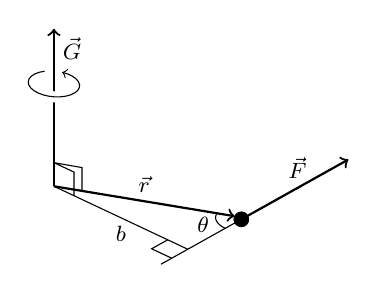
\begin{tikzpicture}[
            z={(0,1)},
            x={(0.85,-0.4)},
            y={(0.8,0.7)}
        ]
            \footnotesize
            \draw [thick,->] (0,0,0) -- (0,0,2) node[below right]{$\vec{G}$};
            \draw [thick,->] (0,0,0) -- node[above]{$\vec{r}$} (1.9,1,0);
            \draw [thick,->] (2,1.1,0) -- node[above]{$\vec{F}$} (2,3,0);
            \fill (2,1,0) circle (1mm);
    
            \draw (0,0,0) -- node[below]{$b$} (2,0,0);
            \draw (2,1,0) -- (2,-0.5,0);
    
            \draw
                (0,0,0.3) -- (0.3,0.15,0.3) -- (0.3,0.15,0)
                (0,0,0.3) -- (0.3,0,0.3) -- (0.3,0,0)
                (1.7,0,0) -- (1.7,-0.3,0) -- (2,-0.3,0)
            ;
    
            \draw [white,line width=4pt] plot [domain=290:320] ([yshift=1.3cm]\x:0.3);
            \draw [->] plot [domain=150:470] ([yshift=1.3cm]\x:0.3);
            \draw plot[domain=200:270] ([xshift=2.38cm,yshift=-0.42cm]\x:0.3);
            \node [left,yshift=-1pt] at ([xshift=2.38cm,yshift=-0.42cm]240:0.3) {$\theta$};
        \end{tikzpicture}
        \caption{Moments.}
        \label{fig:moments}
    \end{figure}
    \begin{itemize}
        \item $\vec{G}$ points in the direction of the axis about which the force tends to rotate the particle, i.e., normal to the plane formed by $\vec{r}$ and $\vec{F}$.
        \item The magnitude of $\vec{G}$:
        \begin{equation*}
            |\vec{G}| = G
            = rF\sin\theta
            = bF
        \end{equation*}
    \end{itemize}
    \item \textbf{Moment about the $\bm{x}$-axis}: The following quantity. \emph{Denoted by} $\bm{G_x}$. \emph{Given by}
    \begin{equation*}
        G_x = yF_z-zF_y
    \end{equation*}
    \item \textbf{Moment about the $\bm{y}$-axis}: The following quantity. \emph{Denoted by} $\bm{G_y}$. \emph{Given by}
    \begin{equation*}
        G_y = zF_x-xF_z
    \end{equation*}
    \item \textbf{Moment about the $\bm{z}$-axis}: The following quantity. \emph{Denoted by} $\bm{G_z}$. \emph{Given by}
    \begin{equation*}
        G_z = xF_y-yF_x
    \end{equation*}
    \item Moments play an important role in rigid body dynamics (see Chapters 8-9).
    \item \textbf{Angular momentum about the origin} (of a particle at position $\vec{r}$ with momentum $\vec{p}$): The vector product defined as follows. \emph{Also known as} \textbf{moment of momentum about the origin} \emph{Denoted by} $\bm{\vec{J}}$. \emph{Given by}
    \begin{equation*}
        \vec{J} = \vec{r}\times\vec{p}
    \end{equation*}
    \begin{itemize}
        \item Alternate form:
        \begin{equation*}
            \vec{J} = m\vec{r}\times\dot{\vec{r}}
        \end{equation*}
    \end{itemize}
    \item \textbf{Angular momentum about the $\bm{x}$-axis}: The following quantity. \emph{Denoted by} $\bm{J_x}$. \emph{Given by}
    \begin{equation*}
        J_x = m(y\dot{z}-z\dot{y})
    \end{equation*}
    \item \textbf{Angular momentum about the $\bm{y}$-axis}: The following quantity. \emph{Denoted by} $\bm{J_y}$. \emph{Given by}
    \begin{equation*}
        J_y = m(z\dot{x}-x\dot{z})
    \end{equation*}
    \item \textbf{Angular momentum about the $\bm{z}$-axis}: The following quantity. \emph{Denoted by} $\bm{J_z}$. \emph{Given by}
    \begin{equation*}
        J_z = m(x\dot{y}-y\dot{x})
    \end{equation*}
    \item \textbf{Momentum}: A quantitative measure of the motion of a moving body. \emph{Also known as} \textbf{linear momentum}. \emph{Denoted by} $\bm{\vec{p}}$. \emph{Given by}
    \begin{equation*}
        \vec{p} = m\vec{v}
    \end{equation*}
    \item The rate of change of the angular momentum is equal to the moment of the applied force:
    \begin{equation*}
        \dot{\vec{J}} = m(\dot{\vec{r}}\times\dot{\vec{r}}+\vec{r}\times\ddot{\vec{r}})
        = 0+\vec{r}\times m\ddot{\vec{r}}
        = \vec{r}\times\vec{F}
        = \vec{G}
    \end{equation*}
    \begin{itemize}
        \item This is analogous to the result that
        \begin{equation*}
            \dot{\vec{p}} = \vec{F}
        \end{equation*}
    \end{itemize}
    \item \textbf{Axial} (vector): A vector whose direction depends on the choice of a right-hand screw convention.
    \item \textbf{Polar} (vector): A vector whose direction does not depend on the choice of a right-hand screw convention.
\end{itemize}


\subsection*{Section 3.4: Central Forces; Conservation of Angular Momentum}
\begin{itemize}
    \item \textbf{Central} (external force): An external force that is always directed toward or away from a fixed point.
    \item \textbf{Center of force}: The fixed point toward or away from which a central force is always pointed.
    \item Whenever possible, we pick the origin as our center of force.
    \begin{itemize}
        \item In this case, $\vec{r}\parallel\vec{F}$, so
        \begin{equation*}
            \vec{G} = \vec{r}\times\vec{F} = 0
        \end{equation*}
        \item The above is a good condition for $\vec{F}$ to be central.
        \item Consequence: Since $0=\vec{G}=\dot{\vec{J}}$ for a central force, $\vec{J}$ is constant under central forces! This observation can be formalized as follows.
    \end{itemize}
    \item \textbf{Law of conservtion of angular momentum}: As long as a particle is subject only to central forces, its angular momentum does not change.
    \begin{itemize}
        \item Note that this implies that both the \emph{direction} and \emph{magnitude} of the angular momentum are conserved in such a situation!
    \end{itemize}
    \item Implications of the conservation of the \emph{direction} of $\vec{J}$.
    \begin{figure}[h!]
        \centering
        \begin{tikzpicture}[
            z={(0,1)},
            x={(0.85,-0.4)},
            y={(0.8,0.7)}
        ]
            \footnotesize
            \draw (-1,-2,0) -- (3,-2,0) -- (3,4,0) -- (-1,4,0) -- cycle;
    
            \draw [rex,thick] plot [domain=0:110] (\x:{5^0.5});
            \draw [white,line width=4pt] (0,0,0) -- (0,0,2);
            \draw [thick,->] (0,0,0) -- node[near end,below left]{$\vec{J}$} (0,0,2);
            \draw [thick,->] (0,0,0) -- node[above]{$\vec{r}$} (1.9,1,0);
            \draw [thick,->] (2,1.1,0) -- node[right]{$\vec{v}$} ++(-1,2,0);
            \fill (2,1,0) circle (1mm);
    
            \draw (0,0,0.3) -- (0.3,0.15,0.3) -- (0.3,0.15,0);
        \end{tikzpicture}
        \caption{The law of conservation of angular momentum.}
        \label{fig:conservAngMtum}
    \end{figure}
    \begin{itemize}
        \item The motion is always confined to a plane, i.e., the plane to which $\vec{J}$ is normal and in which $\vec{r},\vec{p}$ lie.
        \item This is obvious physically (see Figure \ref{fig:conservAngMtum}).
    \end{itemize}
    \item Implications of the conservation of the \emph{magnitude} of $\vec{J}$.
    \begin{itemize}
        \item Since $v_r=\dot{r}$, $v_\theta=r\dot{\theta}$, and $J=mrv_\theta$,\footnote{Why is $v_r$ not included here??} we have that
        \begin{equation*}
            J = mr^2\dot{\theta}
        \end{equation*}
        \item That is, as the radius shrinks, the angular velocity increases and vice versa.
    \end{itemize}
    \item A note on \textbf{Kepler's second law} and sweeping out equal areas during similar time intervals.
\end{itemize}


\subsection*{Section 3.5: Polar Coordinates}
\begin{itemize}
    \item Works out a lot of relevant formulas.
    \item A better way to work all these out is with Lagrangian mechanics!
    \item \textbf{Variational principle}: A principle which states that some quantity has a minimum value or, more generally, a stationary value.
\end{itemize}


\subsection*{Section 3.6: The Calculus of Variations}
\begin{itemize}
    \item Goes through the shortest distance example.
\end{itemize}


\subsection*{Section 3.7: Hamilton's Principle; Lagrange's Equations}
\begin{itemize}
    \item \textbf{Hamilton's principle}: The action integral $I$ is stationary under arbitrary variations $\var{x},\var{y},\var{z}$ which vanish at the limits of integration $t_0,t_1$.
    \item \textbf{Lagrange's equations}: The equations given as follows for $i=1,\dots,n$. \emph{Given by}
    \begin{equation*}
        \dv{t}(\pdv{L}{\dot{q}_i}) = \pdv{L}{q_i}
    \end{equation*}
    \item Conversion factors to other coordinate systems given, e.g., $\pdv*{T}{\dot{\rho}}$ from cylindrical.
\end{itemize}


\subsection*{Section 3.8: Summary}
\begin{itemize}
    \item Some good ideas.
\end{itemize}




\end{document}